% Physics of the 19th century

\documentclass[11pt]{article}

\usepackage[a4paper, margin=1in]{geometry}

\usepackage{amsmath}

\usepackage{amssymb}

\usepackage[german]{babel}

\usepackage[autostyle=true]{csquotes}

\usepackage{libertine}

\usepackage[libertine]{newtxmath}

\usepackage{tikz}

\usepackage{gensymb}

\usepackage{fancyhdr}

\usepackage{amsfonts}

\usepackage{pgfplots}

\pgfplotsset{compat=1.10}

\usepackage{multicol}

\usepackage{caption}

\usepackage{floatrow}

\everymath{\displaystyle}

% Header / footer settings

\pagestyle{fancy}
\fancyhf{}
\renewcommand{\headrulewidth}{0.2mm}
\fancyhead[C]{Funktionen}
\renewcommand{\footrulewidth}{0.2mm}
\fancyfoot[L]{Peter Goldsborough}
\fancyfoot[C]{\thepage}
\fancyfoot[R]{\today}

\fancypagestyle{plain}{%
	\fancyhf{}
	\renewcommand{\headrulewidth}{0mm}%
	\renewcommand{\footrulewidth}{0.2mm}%
	\fancyfoot[L]{Peter Goldsborough}
	\fancyfoot[C]{\thepage}
	\fancyfoot[R]{\today}
}


\setlength{\headheight}{15pt}

\setlength{\parindent}{0pt}

\addtolength{\parskip}{\baselineskip}


\newcommand{\overbar}[1]{\mkern 1.5mu\overline{\mkern-1.5mu#1\mkern-1.5mu}\mkern 1.5mu}

\newcommand{\heading}[1]{\begin{center}\Huge \textbf{#1}\end{center}\par}

\newcommand{\sub}[1]{\vspace{\parskip}{\LARGE\textbf{#1}}}

\newcommand{\subsub}[1]{{\Large \textbf{#1}}}

\newcommand{\subsubsub}[1]{\textbf{#1}}

\newcommand{\colvec}[1]{\begin{pmatrix}#1\end{pmatrix}}

\newcommand{\extrapar}{\par\vspace{\baselineskip}}

\newcommand{\zitat}[1]{\foreignquote{german}{#1}}

\newcommand{\bolditem}[1]{\item \textbf{#1}}

\newcommand{\titleitem}[1]{\bolditem{#1}\par}

\newcommand{\defas}{ \dots \,\,}

\begin{document}
\thispagestyle{plain}

\heading{Physics of the 19th century}

\sub{Lasers}

The word ``laser'' is an acronym for \emph{Light Amplification by Stimulated Emission of Radiation}. Laser light finds many practical applications in everyday life and technology, from basic toy laser-pointers to bar-code product identification systems in supermarkets to CD and DVD drives in computers, audio systems or DVD players. The properties of laser light are explained, examined and discussed in the following paragraphs.

\subsub{Properties of Laser Light}

There are four main properties and terms associated with laser light that set it apart from conventional forms of light from filament lamps or the sun. Laser light is \dots

\begin{itemize}
	
	\bolditem{Monochromatic}: laser light only has one \emph{chroma}, i.e. a single color. The color of light is related to its frequency $f$ and wavelength $\lambda$, thus this property essentially means that all photons in laser light have the same frequency and wavelength. Popular laser colors are red or green.

	\bolditem{Coherent}: all photons of laser light ray have the same phase --- they are \emph{in phase} or \emph{in step}. This is due to the fact that laser photons are not emitted spontaneously as is the case for ordinary, conventional sources of light such as filament lamps, where atoms emit light spontaneously and independently from one another. Rather, laser photons are emitted by explicit stimulation, one after another in a chain-reaction. The coherence adds to the amplitfication of the light due to constructive intereference.

	\bolditem{Collimated}: the light emitted is highly focused and highly directional and is usually only a relatively narrow beam, with little divergence. By comparison, ordinary light from the sun, a candle or a light bulb is not at all \emph{collimated} or focused, but radiates away in many or all directions. This degree of high collimation results from the setup of the cavity of a laser. The material from which light photons are emitted --- often a synthetic ruby crystal --- is placed between two parallel mirrors. One of the two mirrors --- the back mirror --- is entirely reflective, while the other --- the front mirror --- is only around 99 percent reflective, letting through 1 percent as the laser light beam and reflecting the rest. Only light rays perpendicular to the mirrors (parallel to the path between them) are let through, thus they are all in the same direction --- they are \emph{collimated}.

	\bolditem{Intense}: the light is high and approximately uniform in energy density throughout.

\end{itemize}

\subsub{Terminology of Laser Light}

It should be explained what the difference between stimulated and spontaneous emission is, as it is this distinction that makes laser light unique compared to ordinary, conventional sources of light. Furthermore, there are a few other terms that carry an important meaning in association with laser light.

\begin{itemize}

	\titleitem{Spontaneous Emission}

	Spontaneous emission is the phenomenon whereby an excited electron in a higher energy level or quantum state of an atom transitions to a lower state, possibly the ground state of the atom, at a \emph{random} point in time and thereby \emph{spontaneously} emits a light photon whose frequency $f$ depends on the discrete difference in energy $\Delta E$ between the energy of the electron in at initial quantum state and its final energy level, according to the Planck relation which states that the energy $E$ of a photon is equal to $h \cdot f$, where $h$ is Planck's constant and $f$ the photon's frequency. Spontaneous emission is the standard form of emission and produces light that is incoherent (out of phase), polychromatic (many wavelengths, frequencies and colors) and divergent (not collimated).

	\titleitem{Stimulated Emission}

	Stimulated emission is the process whereby an incoming photon, whose energy is equal to the energy difference $\Delta E$ of an electron's current quantum state and a lower energy level, can \emph{stimulate} or \emph{trigger} the transition of the electron from its initial, higher energy state to the final, lower quantum level. As a result, the electron emits an exact, identical copy of the incoming photon such that there are now two photons with the same phase, frequency and direction of travel. Under natural circumstances, stimulated emission is a very rare phenomenon. The reason why is that when an electron absorbs a discrete quantum of energy carried by a photon to reach a higher quantum state (energy level), it remains at this excited state for only a short period of time, around $10^{-8}$ seconds. In this very small time interval, it is highly improbable that a photon carrying just the right, necessary energy will pass the electron to stimulate its transition to a lower quantum state. Population inversion via optical pumping is the method by which laser light increases the chance of stimulated emission. Light produced via stimulated emission is monochromatic (single color and frequency), coherent (equal phase) and collimated (directional and focused) --- perfect for lasers.
	
	\titleitem{Bottom Heavy}

	A material is referred to as being \emph{bottom heavy} when there is a greater number of electrons at the ground state or generally at lower quantum levels compared to the number of electrons in higher excited states. This is the usual case for the majority of solids and materials, as for there to be electrons in higher states an additional input of energy in form of photons is required, which may then be absorbed by electrons to perform a quantum leap to transition to a higher excited state.

	\titleitem{Population Inversion}

	Materials are usually bottom heavy, but under certain circumstances there can be more electrons in higher energy states than there are in lower levels, which is atypical and must therefore be stimulated. This situation is referred to as \emph{population inversion}. The achievement of a significant population inversion in atomic energy states is a precondition for the generation of laser light. For lasers, this population inversion is achieved via \emph{optical pumping}, such that a significant number of electrons is found in the \emph{metastable states} of the material.

	\titleitem{Metastable States}

	Certain elements such as neon or helium or synthetic ruby happen to have certain electron energy states that are longer-lived than ordinary quantum levels. These metastable states can be seen as temporary energy traps. They stil provide less stability than the ground state of an atom, however the time spent by an electron that absorbs the right quantum of energy to reach such a metastable state is still greater than the time spent in an ordinary energy level by a factor $10^4$. All laser materials must have metastable states.

	\titleitem{Optical Pumping}

	The process whereby a light (optical) source is used to ``pump'' or elevate electrons from lower energy levels to higher quantum states. The light source emits photons carrying a quantum of energy that is just right for electrons to absorb them and to reach a \emph{metastable state}. Via optical pumping, population inversion is achieved. At some random point in time, one of the optically pumped electrons will undergo spontaneous emission and thereby emit a photon whose energy is just enough to de-excite neighbouring electrons that are also in the metastable state (which are many, because of population inversion). This causes a chain-reaction of stimulated emission of identical light photons with the same phase and frequency, leading to their superposition and thus \emph{light amplification}.

	\titleitem{Amplifying Medium}

	The amplifying medium refers to the material in which light amplification by stimulated emission of photons takes place. Often, this material may be synthetic ruby, a mixture of helium and neon gases or various possible semiconductors. The essential property of the amplifying medium is that it allows its atoms to have metastable states, which can trap electrons for longer durations and thus make population in version possible.

\end{itemize}

It should quickly be summarized how the above concepts and phenomena lead to an first amplification of coherent and monochromatic light. In the first step, \emph{optical pumping} is used to elevate electrons within the \emph{amplifying medium} to \emph{metastable states}, where they are trapped for durations longer than normal. This makes \emph{population inversion} possible, which is the situation where there are more electrons in higher quantum states than in lower ones, which is atypical as materials are normally \emph{bottom heavy}. When many electrons are in the metastable states, one will spontaneously transition to a lower energy level and thereby emit a photon. Because this photon carries energy that is just the right, discrete quantum of energy required for the other excited electrons in the metastable state to de-excite, this single spontaneously-emitted photon from the first electron causes a chain reaction of stimulated emissions of radiation from other electrons. The light photons emitted in this process are identical copies of one another and are equal in phase (light is coherent) and frequency (light is monochromatic). This is the basic working principle of stimulated emission within the amplifying medium. The light produced is then further amplified by the \emph{laser cavity}, whose setup is explained below.

\subsub{Setup of a Laser Cavity}

After initial generation of coherent and monochromatic light via stimulated emission within the amplifying medium, the light is further amplified in the \emph{laser cavity}. For this, the amplifying medium is placed between two parallel mirrors, one of which is completely ($\sim 100\%$) reflective --- the back mirror --- while the other is partially ($\sim 99\%$) reflective --- the front mirror. The purpose of these mirrors is to bounce photons back and forth within the laser cavity to achieve more stimulated emission of light photons. About one percent of the light leaves the front, partially reflective mirror as the output of the laser --- the light you see. There are two further advantages of the laser cavity setup with the two mirrors:

\begin{enumerate}
	
	\item The mirrors are setup parallel to one one another, at either end of the laser cavity. There is no reflective medium above or below the cavity, thus only light that is perpendicular to the mirrors is reflected, while all other directions of light that would not improve the collimation of the light but rather increase its divergence are simply absorbed by whatever is above or below the cavity.

	\item An optical standing wave is created with two nodes at either mirror. This leads to a filtering and selection of the frequency as the light photons emitted by the amplifying medium cover a small range of frequencies --- the photons are not perfectly monochromatic. The standing narrow this range to improve the degree of how monochromatic the light is.

\end{enumerate}

\subsub{Applications of Laser Light}

Two real-world applications of laser-light are examined further in this section.

\subsubsub{Bar Codes}

Bar codes are used in supermarkets, libraries or or warehouses to identify object, products or other items. They are a very simple application of laser light. For a bar code, the thickness of each of the black lines codes for a digit between 0 and 9. A laser scans over the bar code, while a suitable photodetector measures how much of the light emitted from the scanner, hitting each individual line, is reflected back to the scanner. The thicker the line, the more it will absorb the light and the less it will reflect. This determines the digit. The white space between the digits does not absorb light as much.

\begin{figure}[h!]
	\centering
	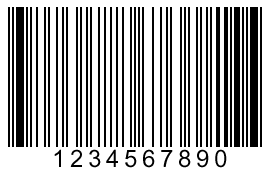
\includegraphics[scale=0.8]{img/bar}
	\caption*{A Bar Code}
\end{figure}

\subsubsub{Optical Drives}

Optical drives are the components of DVD players or computers that read information and data stored on compact discs (CDs) or digital versatile discs (DVDs). They utilize lasers in a most interesting way. Collimated, coherent and monochromatic light from a laser is emitted onto the surface of a CD (everything will also apply to a DVD) that is composed of many small pits spaced apart at a certain distance, but all one quarter of the wavelength of the laser light \emph{deep} (going into the surface layer of the CD by one fourth of the wavelength). When light passes over a plateau, i.e. a region on the CD that is not a pit (always between two pits), or right into a pit, the light will be reflected with full intensity (also constructive interference with incoming light) and this will be detected by a photodetector in the reading device and interpreted as a HIGH signal (binary 1). However, when the light falls right onto the edge of a pit and plateau, the light travelling down the pit will be reflected and interfere with the light reflected at the plateau $180\degree$ later in its cycle. More precisely, the light travels one fourth of a wavelength down the pit and another fourth on the way back to meet up with the plateau light at a phase difference of $180\degree$. This results in destructive intereference and a loss in intensity which is once more detected by the photodetector and this time interpreted as a LOW signal (binary 0). The binary sequence of the data stored on the CD is then converted into analog via a suitable digital-to-analog converter (DAC).

\begin{plot}

	% CD Surface
	\draw (0, 0)
	 -- ++(2, 0) node [midway, above] {Pit}
	 -- ++(0, 1) node [midway, left] {$\frac{\lambda}{4}$}
	 -- ++(1, 0) -- ++(0, -1)
	 -- ++(2, 0) node [midway, below] {CD Surface}
	 -- ++(0, 1) -- ++(1, 0) -- ++(0, -1) -- ++(2, 0);

	 % Plateau label
	 \draw [->] (2, -0.5) node [below] {Plateau} -- (2.5, 0.5);

	% High signal
	\draw [red, line width=0.5cm]
	      (4, 2.5) -- (4, 0) node [pos=0.3, left, black] {HIGH};

	% Low signal
	\draw [red, line width=0.25cm]
	      (5.875, 2.5) -- ++(0, -1.5);

	\draw [red, line width=0.25cm]
	      (6.125, 2.5) -- ++(0, -2.5) node [pos=0.3, right, black] {LOW};

\end{plot}

\sub{Quantum Mechanics}

Quantum mechanics is the branch of physics that deals with the physical phenomena as well as the description of the motion and interaction of subatomic particles at the nanoscopic, atomic scale. It incorporates the concepts of quantization of energy, i.e. the observation that certain physical quantities, such as the energy of electrons, can only change in \emph{discrete} amounts (\emph{quanta}) and not in a continuous way. Important concepts include the wave-particle duality of light and matter as well as the Heisenberg uncertainty principle.

\subsub{The Photoelectric Effect}

At the end and beginning of the 19th century, the dominant theory governing the description of the motion and properties of light and its interactions with the physical world was based on the assumption that light travels as a wave. The characteristics of a wave include that it has a certain frequency $f$, a wavelength $\lambda$, an amplitude $A$ and an intensity $I = A^2$ as well as the fact that it can undergo reflection, refraction, polarization, dispersion and can diffract, superpose, interfere and thereby create an interference pattern. These properties were all observed for light. However, there was one experiment and one phenomenon that could not be explained by the wave theory of light: the photoelectric effect. The photoelectric effect is the the observation that many metals emit electrons --- then called \emph{photoelectrons} --- when light shines upon them. This phenomenon was first discovered by Wilhelm Hallwachs in 1888 but observed before that by Heinrich Hertz, which is why the photoelectric effect is less commonly referred to as the \emph{Hertz effect}.

\subsubsub{Setup}

The basic experimental setup of an experiment to observe the photoelectric effect involves a simple electric circuit containing a negatively charged metal plate as well as a positively charged anode inside a vacuum tube, connected to a battery. This metal is most commonly zinc, though sodium or copper may also be used, especially to understand and investigate how the choice of metal influences the results of the photoelectric effect. Moreover, there must a light source with variable intensity and a control to vary the frequency or wavelength of the light emitted. A certain potential difference is kept across the two plates by a battery or some other form of power supply.

\begin{circuit}
	
	% Negatively charged cathode
	\draw [line width=0.08cm] (0, -1) -- ++(0, 2);

	% Positively charged anode
	\draw [line width=0.08cm] (4, -1) -- ++(0, 2);

	% Circuit
	\draw (4, 0)
	 -- ++(1, 0)
	 -- ++(0, -2.5)
	 	  to [ammeter] ++(-3, 0)
	      to [battery] ++(-3, 0)
     -- ++(0, 2.5)
     -- ++(1, 0);

    % Charges
    \foreach \i in {-0.8, -0.5, -0.2, 0.2, 0.5, 0.8}
    {
    	% Negative at cathode
    	\draw [blue] (-0.2, \i) node {$-$};

    	% Positive at anode
    	\draw [red] (4.2, \i) node {$+$};
    }

    % Light source
    \draw [very thick, rotate=-40]
          (0.5, 3)
     -- ++(1, 0)
     -- ++(130:0.5)
     -- ++(0, 0.8)
     -- ++(-0.35, 0)
     -- ++(0, -0.8)
     -- ++(230:0.5);

\end{circuit}

According to the classical theory of light, were light to be emitted by the light source in the direction of the negatively charged plate, the \emph{intensity} of the light (the square of its amplitude) would influence the rate of emission of electrons as well as the kinetic energy of the electrons freed from the atoms they are bound to in the metallic lattice of the metal plate. The frequency or wavelength would play no role at all, thus it would be expected that the same results are observed for ultraviolet light, visible light, infrared light or any other frequency and wavelength on the electromagnetic spectrum. However, this was not proven true during the various experiments undertaken to understand the photoelectric effect. When illuminated with ultraviolet light of a certain wavelength, electrons would be emitted from the metal plate, causing a current to be detected by the ammeter. However, when the illumination was repeated with light in the visible range of the electromagnetic spectrum ($\sim 700$ nm to $\sim 400$ nm), there was no emission of electrons observed --- the reading of the ammeter remained zero.

A scientist named Philipp Lenard made initial observations about this effect and defined a set of laws of photoelectrics: 

\begin{itemize}
	
	\item For any metal, electrons are emitted only if the frequency of the indicent light is greater than some threshold value $f_0$ -- the cut-off or threshold frequency. Therefore, weak ultraviolet light could cause emission of electrons from a zinc plate, while very intense infrared light could not.

	\item The threshold frequency $f_0$ is different for different materials and depends on the \emph{reactivity} of the elemental make-up of the metal.

	\item The kinetic energy of the electrons emitted is independent from the intensity of the incident radiation and depends solely on its frequency. The maximum kinetic energy of the ejected electrons is proportional to the difference between the light frequency $f$ and the threshold frequency $f_0$: $$E_{kin} \propto (f - f_0)$$

	\item The intensity of the light source does not influence the kinetic energy of the electrons emitted, nor whether or not electrons are emitted in the first place. If electrons are emitted at a certain wavelength of light, then the intensity does, however, influence the \emph{number} of photoelectrons emitted and thus the current flowing between the plates.

\end{itemize}

While Philipp Lenard made important observation concerning the photoelectric effect, he could not yet explain its cause. This was done by a greater mind, Albert Einstein, for which he received the Nobel Prize in 1921. Einstein built his explanation on work done by fellow German physicist Max Planck, who had already proposed that electromagnetic radiation such as light was always emitted in \emph{discrete energy packets} or \emph{quanta}, later then called \emph{photons}. Albert Einstein found that all experimental laws defined by Lenard could thus be explained if it is was assumed that atoms can only absorb light in discrete amounts --- \emph{quanta} --- and that the magnitude of one such quantum of energy is proportional to the frequency of the light, as given by the \emph{Planck relation} of frequency $f$ and energy $E$: $$E = h \cdot f$$ This revolutionary explanation, indicating that the phenomenon of light could not be explained entirely by the wave model, initiated one of the most important paradigm shifts in physics. Einstein proposed the following assumptions regarding photons:

\begin{itemize}
	
	\item Photons are discrete, quantized packets of energy that are indivsible, such that a photon may transfer either all of its energy or none at all. 

	\item All metals are characterized by a certain minimum or threshold energy required to eject electrons from the atoms within its metallic lattice. This threshold energy is referred to as the \emph{work function} $\phi$ of the metal and is defined as the miniminum energy required to free electrons from its surface. The value of this work function is dependent on the threshold frequency $f_0$ of the metal according to the Planck relation: $\phi = h \cdot f_0$. Different metals have different work function values that depend on the reactivity of the metal. As an example, the work function $\phi$ of zinc is approximately $4.3\, eV$, thus its threshold frequency $f_0$ is equal to about $10^{15} Hz$. 

	\item A photon of light emitted from the light source will only result in the ejection of an electron if its frequency $f$ is greater than the threshold frequency $f_0$ and thus if its energy $E = h \cdot f$ is greater than the work function $\phi = h \cdot f_0$. Once the photon frequency trespasses the threshold set by the work function of the metal, the maximum kinetic energy $E_{kin}$ of the electron emitted is \emph{proportional} to the difference $f - f_0$ between the frequency of the photon and the threshold frequency, while it is (less than or) \emph{equal} to the difference $E - W$ between the energy of the photon and the minimum energy required to free an electron. Thus it can be said that once the energy suffices, the kinetic energy of the electrons emitted from the metal is equal to the excess energy of the photons: $$E_{kin} = E - \phi = h \cdot (f - f_0) \text{ given that } f > f_0 \text{ and } E > \phi$$

	\item Increasing the intensity does not affect the energy of individual photons, nor the kinetic energy of the photoelectrons emitted (if any), but influences only the \emph{number} of photons ejected by the light source. If the frequency $f$ of the photons emitted from the light source is greater than the threshold frequency $f_0$, such that the discrete quanta of energy $E$ they carry is greater than the work function $\phi$ of the metal, then one photon of light will cause exactly one electron to be emitted from the metal. An increase in the intensity of the light source then results in more photons being emitted and thus more electrons being freed from the atoms within the metallic lattice of the plate. If, however, the frequency and energy of the photons is not sufficient, i.e. not greater than $f_0$ and $\phi$, respectively, then it is entirely irrelevant how many photons are emitted from the light source (how intense the light is), as none will carry the required, minimum, discrete quantum of energy required to free and eject a single electron. Thus, in conclusion, three cases can be defined for the effect of the size of the energy $E$ of the photons emitted from the light source, relative to the work function $\phi$:

	\begin{enumerate}

		\item If $E - \phi < 0$ such that $E$ is less than the minimum required energy to free an electron, then the electron will not be ejected. Current does not flow.

		\item If $E - \phi = 0$ such that $E$ equals the work function $\phi$, then the electron will be freed but without kinetic energy. Current does not flow.

		\item If $E - \phi > 0$ such that $f$ is greater than the threshold frequency $f_0$, an atom will be ionized and the kinetic energy of the electron emitted will be equal to the excess energy of the photon $E - \phi$. Current flows.

	\end{enumerate}

\end{itemize}

\begin{figure}[h!]
	\centering
	\begin{tikzpicture}

		% Kinetic energy of photoelectrons axis
		\draw [<->] (0, -2) -- ++(0, 6)
		      node [midway, rotate=90, above]
		      {Kinetic Energy of Photoelectrons}
		      node [right] {$E(f) = h \cdot f$};

		% Photon-frequency axis
		\draw [->] (0, 0) -- ++(7, 0)
		      node [below, pos=0.75] {Frequency of Photons}
		      node [pos={9/35}] {$|$};

		% Threshold frequency label
		\draw (1.8, -0.5) node [red] {$f_0$};

		% Graph
		\draw [domain=0:6] plot (\x, {5/6 * \x - 1.5});

		% Slope (h)
		\draw (3.5, 2) node [rotate=40] {Slope is Planck's constant $h$};

	\end{tikzpicture}
	\caption*{A generalized graph plotting photoelectron-energy in dependence of photon-frequency for a given metal of threshold frequency $f_0$}
\end{figure}

\pagebreak

\subsub{Matter Waves and the Wave-Particle Duality}

The most important conclusion Einstein derived from the photoelectric effect was that light has both wave-like properties, such as a frequency, wavelength and the fact that it diffracts, refracts, reflects or disperses, as well as particle-light properties, such as the ability to carry discrete amounts of energy as well as have a certain \emph{linear momentum}. This is what is described as the \emph{wave-particle} duality of light, which Albert Einstein commented on with the following words:

\begin{displayquote}

	It seems as though we must use sometimes the one theory and sometimes the other, while at times we may use either. We are faced with a new kind of difficulty. We have two contradictory pictures of reality; separately neither of them fully explains the phenomena of light, but together they do.

\end{displayquote}


A French physicist called Louis de Broglie thereafter proposed that if light has both wave and particle-light characteristics, also particles and all matter must display wave-like properties, alongside their natural particle qualities. This became known as the \emph{de Broglie hypothesis}, formulated in 1924, and eventually as the \emph{wave-particle duality} of matter. De Broglie's argument was composed of three main observations:

\begin{enumerate}
	
	\item Wave-like properties of light are determined by a wavelength $\lambda$

	\item Particle-like properties are fixed by a linear momentum $p = m \cdot v$

	\item These can be linked for a photon according to Einstein's mass-energy relation $E = m \cdot c^2$ and his (or Planck's) energy-frequency relation $E = h \cdot f$ as well as the definition of photon momentum $p$ as being equal to the product of its mass $m$ times the speed of light $c$ in the following way: $$E = h \cdot f = m \cdot c^2 \AND p = m \cdot c \AND c = \lambda \cdot f$$ $$\Downarrow$$ $$p = m \cdot c = \frac{h \cdot f \cdot c}{c^2} = \frac{h \cdot f}{c} = \frac{h \cdot f}{\lambda \cdot f} = \frac{h}{\lambda}$$ $$\Downarrow$$ $$p = \frac{h}{\lambda} \AND \lambda = \frac{h}{p}$$

\end{enumerate}

The wavelength $\lambda$ of a particle can thus be expressed as Planck's constant $h$ divided by the linear momentum $p = m \cdot v$ of the particle (where its speed or velocity $v$ is fixed as the speed of light). This wavelength is known as the \emph{de Broglie wavelength}. This relationship can be expanded further to see that the particle's wavelength stands also in relation to its kinetic energy $E_{kin}$: $$E_{kin} = \frac{m \cdot v^2}{2} \thus E_{kin} =  \frac{p^2}{2 \cdot m} \thus p = \sqrt{2 \cdot m \cdot E_{kin}}$$ $$\Downarrow$$ $$\lambda = \frac{h}{p} = \frac{h}{\sqrt{2 \cdot m \cdot E_{kin}}}$$

\pagebreak

\subsubsub{Proof of the de Broglie Hypothesis and Particle Diffraction}

If the de Broglie hypothesis were true and particles were to have wave-like properties, they would also have to be able to diffract, i.e. spread out in a circular fashion as they pass through gaps equal or similar in size to their wavelength, and subsequently, when multiple waves superpose, show an interference pattern with maxima and minima. This was indeed proven in 1927 by the American scientists Clinton Davisson and Edmund Germer, who sucessfully directed electron beams at a nickel crystal to prove that they created an interference pattern. The setup of this experiment included the following components:

\begin{itemize}

	\item A negatively charged, heated \textbf{electron gun} that releases thermally excited electrons.

	\item An \textbf{accelerating anode} connected to a variable resistor (potentiometer), so that a variable potential difference could be established across the heated electron gun (the cathode) and the anode to accelerate excited electrons.

	\item A \textbf{crystalline nickel target}, whose regular arrangement and uniform spacing of atoms (a lattice) acts as a diffraction grating for the electrons. The spacing $d$ between the nickel atoms is approximately $0.215$ nanometers wide.

	\item A \textbf{Faraday Cup} that detects and counts charged particles and is movable along an arc path. 

	\item A \textbf{vacuum chamber} in which the nickel target and the movable detector are placed to ensure that accelerated electrons do not collide with other atoms or molecules in the air.

\end{itemize}

\begin{plot}
	
	% Circuit with heated cathode and accelerating anode
	\draw (0, 0)
	      to [battery] ++(1.5, 0)
	 -- ++(0, 1.5)
	 	  to [potentiometer] ++(-1.5, 0)
	 -- ++(0, -1.5)
	    ++(0, 0.75)
	 -- ++(-2, 0)
	 -- ++(0, 2)
	 -- ++(0.5, 0)
	 -- ++(0, 0.25)
	 -- ++(1.5, 0)
	 -- ++(0, -0.5)
	 -- ++(-1.5, 0) node [above, midway] {Cathode}
	 -- ++(0, 0.25)
	      (0.75, 1.7)
	 -- ++(0, 0.5)
	 -- ++(1, 0)
	 -- ++(0, 0.25)
	 -- ++(-1, 0)
	 -- ++(0, 0.1)
	    ++(0, 0.3)
	 -- ++(0, 0.1)
	 -- ++(2, 0) node [midway, above] {Anode}
	 -- ++(0, -0.1)
	    ++(0, -0.3)
	 -- ++(0, -0.1)
	 -- ++(-1, 0);

	% Vacuum chamber
	\draw (0.3, 2)
	 -- ++(0, 5)
	 -- ++(8, 0) node [pos=0.8, below] {Vacuum Chamber}
	 -- ++(0, -5)
	 -- ++(-8, 0);

	% Nickel target
	\draw (6.2, 2)
	 -- ++(0, 2)
	 -- ++(0.75, 0)
	 -- ++(0, -2) node [midway, right, align=center] {Nickel\\ Target};

	% Detection arc
	\draw [dashed] (2, 4) arc (160:120:5);

	% Faraday cup (movable detector)
	\draw [rotate=45, very thick]
	      (5.8, 1.5)
	 -- ++(0, 0.75)
	 -- ++(0.35, 0) node [midway, above left, align=center] {Movable\\Detector}
	 -- ++(0, -0.75)
	 -- ++(-0.35, 0);

	% Electron beam from electron gun
	\draw [blue, dashed, very thick]
	      (0, 2.7)
	 -- ++(6.2, 0) node [pos=0.75, black, below] {Electron Beam}
	 -- ++(139:4);

	% Angle theta arc
	\draw (4.7, 2.7) arc (180:139:1.5);

	% Angle theta
	\draw (5.2, 3.1) node {\Large $\theta$};

\end{plot}

The analysis of the interference pattern and the determination of minima and maxima of diffracted electrons was then achieved via the following steps:

\begin{enumerate}

	\item A certain potential difference is setup across the electron gun and the accelerating anode. This voltage influences the interference pattern created. Davisson and Germer determined that maximum constructive interference occured at a voltage of $54\, V$.

	\item Thermally emitted electrons are accelerated towards the nickel target, which acts as a diffraction grating. The distance $d$ between the atoms in the metallic lattice of the nickel crystal is equal to $0.215$ nanometers.

	\item Electrons are diffracted and then deflected in a way that the angle $\theta$ at which the faraday cup detects them determines the angle of diffraction.

	\item The movable detector is varied in position across the arc to count electrons. This count varied and showed distinct maxima and minima positions that are typical of a wave intereference pattern.

\end{enumerate}

The wavelength $\lambda$ of the particle (or wave ?) at the $n$-th maximum given the angle of diffraction $\theta$ can be calculated with the following equation: $$d \cdot \sin \theta = n \cdot \lambda$$ The first maximum ($n = 1$) was found at $\theta = 50\degree$, thus the wavelength of an electron must be: $$\lambda = 0.215 \cdot \sin 50 \approx 0.165\, nm$$ It was thus succesfully shown that electrons can diffract and produce an interference pattern, something that previously attributed only to waves. The de Broglie hypothesis of the wave-particle duality of particles and matter was therefore proven true. Moreover, in 1999, Arndt and Zeilinger conducted an experiment at the University of Vienna which showed that even large $C_{60}$ molecules could diffract and produce an interference pattern when directed through a diffraction grating. At this level, it is very difficult to analyse the interference pattern, as maxima and minima come very close to one another.

\subsub{The Double Slit Experiment}

Davisson and Germer proved the de Broglie hypothesis and showed that electrons --- particles --- could diffract and create an interference pattern. However, another experiment, called the \emph{double slit experiment}, made the truly complex nature of quantum mechanics clear. To begin the discussion of the double slit experiment for particles, one should first make an analogy for the problem at hand by examining how large pieces of matter such as marbles act when passing through a single slit. To do so, imagine some source of marbles is set at a certain distance to the slit, behind which a detector screen is placed. When the source begins to eject marbles towards the slit, some will pass through the slit and create a \emph{single band} at the back screen. Not all will travel towards the screen in a straight path, as some hit the inside of the slit at a certain angle and are thus deflected away from the center. But, in general, the pattern produced will be a relatively narrow band as shown below.

\begin{figure}[h!]
	\centering
	\begin{tikzpicture}

		% Source
		\draw [fill=black] (0, 0) circle [radius=1.2pt] node [left] {Source};

		% Slit screen
		\draw [thick]
		      (2, -1)
		 -- ++(0, 0.9)
		    ++(0, 0.2)
         -- ++(0, 0.9) node [above] {Single Slit};

        % Back Screen
        \draw [thick]
              (4, -1) node [below, align=center] {Detector\\ Screen}
         -- ++(0, 2);

        % Stream
        \draw [dashed] (0, 0) -- ++(4, 0);

	\end{tikzpicture}
	%
	\hspace{1cm}
	%
	\begin{tikzpicture}

		% Screen
		\draw (0, 0) -- ++(5, 0) -- ++(0, 3) -- ++(-5, 0) -- ++(0, -3);

		% Spacer
		\draw (0, -0.5);

		% Spots
		\foreach \i in {2.8, 2.7, ..., 0.2}
		{
			\draw [fill=black] ({2.5 + rand * 0.2}, \i) circle [radius=1pt];
		}

	\end{tikzpicture}
	\caption*{The setup is depicted on the left, while the right image displays the pattern produced.}
\end{figure}

\pagebreak

If now a second slit is added to the slit screen, another band is produced. This is the predictable behaviour of matter.
 
\begin{figure}[h!]
	\centering
	\begin{tikzpicture}

		% Source
		\draw [fill=black] (0, 0) circle [radius=1.2pt] node [left] {Source};

		% Slit screen
		\draw [thick]
		      (2, -1)
		 -- ++(0, 0.6)
		    ++(0, 0.2)
		 -- ++(0, 0.4)
		    ++(0, 0.2)
         -- ++(0, 0.6) node [above] {Two Slits};

        % Back Screen
        \draw [thick]
              (4, -1) node [below, align=center] {Detector\\ Screen}
         -- ++(0, 2);

        % First Stream
        \draw [dashed] (0, 0) -- ++(2, -0.3) -- ++(2, 0);

        % Second Stream
        \draw [dashed] (0, 0) -- ++(2, 0.3) -- ++(2, 0);

	\end{tikzpicture}
	%
	\hspace{1cm}
	%
	\begin{tikzpicture}

		% Screen
		\draw (0, 0) -- ++(5, 0) -- ++(0, 3) -- ++(-5, 0) -- ++(0, -3);

		% Spacer
		\draw (0, -0.5);

		% Spots
		\foreach \i in {2.8, 2.7, ..., 0.2}
		{
			\draw [fill=black] ({2 + rand * 0.2}, \i) circle [radius=1pt];

			\draw [fill=black] ({3 + rand * 0.2}, \i) circle [radius=1pt];
		}

	\end{tikzpicture}
	\caption*{The setup is depicted on the left, while the right image displays the pattern produced.}
\end{figure}

We have now investigated the behaviour of particles (matter) in a double slit experiment, with little spectacular behaviour. Next, it should be examined how water waves behave in this experiment. This will prove a little more interesting, as all waves are characterized by the fact that they \emph{diffract} (spread out) when passing through gaps of a size similar to their wavelength $\lambda$. This property of diffraction can be observed very well when letting water waves pass through a single slit. The waves will reach the slit, diffract and radiate outwards circularly. The pattern created at the detection screen shows a single \emph{maximum} at the point of the screen that is closest to the slit, while it decays in intensity in either direction from the maximum. This is due to the fact that waves lose intensity as they travel, meaning maxima are formed where the waves have to travel least and thus lose least intensity, while a greater distance (the further away from the maximum) will cause a loss in intensity, as can be seen by the pattern produced.

\begin{figure}[h!]
	\centering
	\begin{tikzpicture}

		% Source
		\draw [fill=black] (0, 0) circle [radius=1.2pt] node [left] {Source};

		% Slit screen
		\draw [thick]
		      (2, -1)
		 -- ++(0, 0.9)
		    ++(0, 0.2)
         -- ++(0, 0.9) node [above] {Single Slit};

        % Back Screen
        \draw [thick]
              (4, -1) node [below, align=center] {Detector\\ Screen}
         -- ++(0, 2);

        % Stream
        \foreach \i in {0.2, 0.4, ..., 1}
        {
        	\draw (0.2, {-\i * 7/8}) arc (-80:80:\i);
        }

        % Diffracted Stream
        \foreach \i in {0.2, 0.4, ..., 1}
        {
        	\draw (2.2, {-\i * 7/8}) arc (-80:80:\i);
        }

	\end{tikzpicture}
	%
	\hspace{1cm}
	%
	\begin{tikzpicture}

		% Screen
		\draw (0, 0) -- ++(5, 0) -- ++(0, 3) -- ++(-5, 0) -- ++(0, -3);

		% Spacer
		\draw (0, -0.5);

		% Pattern, first part
		\shade [left color=white, right color=black!50!white]
		       (0, 0) rectangle (2.51, 3);

		% Pattern, second part
		\shade [right color=white, left color=black!50!white]
		       (5, 0) rectangle (2.49, 3);

	\end{tikzpicture}
	\caption*{The setup is depicted on the left, while the right image displays the pattern produced.}
\end{figure}

For two slits, the waves will interfere either constructively or destructively. Where peaks meet peaks, the waves amplify. Where troughs meet peaks, the waves cancel. This produces many maxima that decay in intensity in either direction from the center (due to overall loss of intensity in these regions because of their distance), rather than just one in the center. What is produced is called an \emph{intereference pattern}, with several \emph{fringes} (bands of colors).

\begin{figure}[h!]
	\centering
	\begin{tikzpicture}

		% Source
		\draw [fill=black] (0, 0) circle [radius=1.2pt] node [left] {Source};

		% Slit screen
		\draw [thick]
		      (2, -1) node [below] {Two Slits}
		 -- ++(0, 0.6)
		    ++(0, 0.2)
		 -- ++(0, 0.4)
		    ++(0, 0.2)
         -- ++(0, 0.6);

        % Back Screen
        \draw [thick]
              (4, -1) node [below, align=center] {Detector\\ Screen}
         -- ++(0, 2);

        % Stream
        \foreach \i in {0.2, 0.4, ..., 1}
        {
        	\draw (0.2, {-\i * 7/8}) arc (-80:80:\i);
        }

        % Diffracted stream
        \foreach \i in {0.2, 0.4, ..., 1}
        {
        	\draw [red] (2.2, {-\i * 7/8 + 0.2}) arc (-80:80:\i);

        	\draw [blue] (2.2, {-\i * 7/8 - 0.2}) arc (-80:80:\i);
        }

	\end{tikzpicture}
	%
	\hspace{1cm}
	%
	\begin{tikzpicture}

		% Screen
		\draw (0, 0) -- ++(5, 0) -- ++(0, 3) -- ++(-5, 0) -- ++(0, -3);

		% Spacer
		\draw (0, -0.5);

		% Pattern
		\foreach \x/\i in {0/20, 1/40, 2/60}
		{
			\shade [left color=white, right color=black!\i!white]
		           (\x, 0) rectangle ({\x + 0.5}, 3);

		    \shade [right color=white, left color=black!\i!white]
		           ({\x + 0.5}, 0) rectangle ({\x + 1}, 3);

		    \shade [right color=white, left color=black!\i!white]
		           ({5 - \x}, 0) rectangle ({4.5 - \x}, 3);

		    \shade [left color=white, right color=black!\i!white]
		           ({4.5 - \x}, 0) rectangle ({4 - \x}, 3);
		}

	\end{tikzpicture}
	\caption*{The setup is depicted on the left, while the right image displays the pattern produced.}
\end{figure}

\pagebreak

It was now described how particles on the macroscopic scale --- speaking in relative terms --- behave in a one or two-slit experiment. One slit causes one band. Two slits cause two bands. Also, it was described how waves behave. One slit causes one maximum. Two slits cause an interference pattern of many maxima and minima. On the nanoscopic scale, however, the laws of classical mechanics are replaced (or extended) by those of quantum mechanics. This leads to an interesting problem, as will be shown. First, it must be questioned how electrons (or other particles at the atomic or subatomic scale) behave in the case of a single slit. The answer is: identical to large particles. One slit causes one band of particles detected at the back screen. With two slits, however, the astonishing happens: a stream of electrons --- particles (as was thought) --- produce an interference pattern. This caused an uproar in the scientific community at the time this was discovered. Scientists thought to explain this discovery by arguing that the particles would interact physically, bounce off one another and thus coordinate such a pattern. Thus, to investigate the matter further, single electrons were emitted towards the two slits, one at a time. Still, an intereference pattern was created. The conclusion of this was that single electrons ejected from the source must near the two slits, split or change into a wave (of \emph{potentials}), propagate through both slits and finally interfere with itself once more to hit the wall and produce the intereference pattern so typical of waves. Mathematically, however, this phenomenon is even more complex. At the same time, the particle can be found to go through both slits and neither, through only one and through only the other. These states are said to be in \emph{superposition} with each other.

This called for further examination. The call was answered and it was thought that the phenomenon of electron diffraction could be understood by adding a detector to the system, that was to observe through which of the two slits the electron was going at a time. This worked, but the results were even stranger. The detector found that around half the time, an electron would go through the one slit and around half the time it would go through the other. But the result of this was that the electron no longer produced a wave-like interference pattern, but now created two particle-like bands! Simply observing the phenomenon collapsed the creation of the interference pattern and changed the properties of the electron. How was this to be explained?

\subsub{The Wave Function}

The anwer is in the title of this subsection. To explain the underlying concepts of the wave-particle duality of matter, a certain \emph{wave function} $\Psi$ is used. To re-cap, the wave-particle duality refers to the observation that neither the wave model nor the the particle model can be used to consistently explain the behaviour of light or matter under all circumstances. Quantum mechanics, a set of abstract mathematical models, does its best to provide a certain explanation and the wave function $\Psi$ is an integral part of it. A wave function describes the quantum state of a system of one or more particle and is currently the most complete description of matter or radiation. $\Psi$ is essentially a probability distribution or probability density function in the sense that the probability of finding a certain particle at a certain place, at a certain time is linked or proportional to the \emph{intensity} --- the square of the amplitude --- of the wave function. More precisely, the probability of finding a particle in a certain volume of space $dV$ can be found by multiplying the intensity of the wave function by the volume: $$P = |\Psi|^2 dV$$ Given the general nature of a probability distribution, the probability of finding a particle at \emph{any} point in space (the universe) must be equal to $1$, i.e. the particle certainly does exist somewhere. One of the most interesting properties of the wave function, associated with the double slit experiment, is that it \emph{collapses} when a particle in the system governed by the wave function is observed. This explains why electrons only cause an interference pattern when no observer is present, while they go back to producing two bands similar to tennis balls or marbles when observing their motion and behaviour.

\pagebreak

\subsub{The Heisenberg Uncertainty Principle}

One of the most intriguing properties of the wave function is that it collapses and changes continuously. When we try to measure the properties of a matter wave, i.e. its wavelength $\lambda$ or its momentum $p = m \cdot v$, we are forced to interact with it and are thus forced to affect it, to change it. This arises from the wave properties inherent in the quantum mechanical description of nature. Werner Heisenberg, a German scientist, built on this observation in the early 20th century and formulated what is known as the \emph{Heisenberg uncertainty principle}. More precisely, there are two main variants of the uncertainty principle: one of energy and time and one of linear momentum and position. The fundamental law governing both is the following:

\begin{displayquote}
	
	There is a fundamental limit of possible accuracy of measurements.	

\end{displayquote}

\subsubsub{The Uncertainty Principle of Position and Linear Momentum}

The first of the two uncertainty princples concerns itself with the position and linear momentum of a particle, stating that it is not possible to determine both with the same degree of exact precision at the same instant of time. Moreover, Werner Heisenberg proved that the deviation or \emph{uncertainty} in position $\Delta x$ of the particle multiplied by the uncertainty in its linear momentum $\Delta p$ at the same moment could not be less than $\hslash$ divided by two, where $\hslash$ is the reduced Planck's constant and equal to $h$ divided by $2 \pi$: $$\Delta x \cdot \Delta p \geq \frac{\hslash}{2}$$ What this means in practice is that if you were to eject an electron towards a single slit to measure its properties, there would arise two possible scenarios in which the uncertainty principle of position and linear momentum poses problems. In the first case, one may want to determine the position of the electron within the slit precisely. To do so, one would decrease the width of the slit as much as possible. Now, it could be measured with a high level of precision where the electron passes through the slit, as there is simply less room for deviation. Thus, $\Delta x$ would be small. However, at the same time, a decreased gap size results in a higher degree of diffraction, such that the uncertainty of the velocity or linear momentum $\Delta p$ of the particle would be high. The more you want to measure or observe where the particle passes through the slit, the less you know in which direction it will travel. On the other hand, one may want to determine the linear momentum of the particle as precisely as possible. Now, one would increase the gap size to ensure that the particle is diffracted as little as possible. Consequently, $\Delta p$ will be small --- the particle will move on in a predictable direction. At the same time, however, it would have become increasingly difficult to determine the particle's exact position in the slit, as there is more room for uncertainty. In effect, $\Delta x \cdot \Delta p$ will always exceed $\frac{h}{4 \pi}$.

\subsubsub{The Uncertainty Principle of Energy and Time}

The second ucnertainty principle proposed by Heisenberg was that of energy and time. Once more, he argued that the uncertainty $\Delta E$ in energy of a particle multiplied by the uncertainty $\Delta t$ in the time of measurement could not be less than the reduced Planck's constant $\hslash$ divided by two: $$\Delta E \cdot \Delta t \geq \frac{\hslash}{2}$$ The basic principle of this concept and equation is that to measure the energy of a particle at any given point in time precisely, one would need a considerable amount (or span) of time to perform that measurement. Therefore, $\Delta E$ would be small, as the measurement would not deviate much from the actual value, given the large measurement period. However, it would be impossible to say precisely at what \emph{precise} instant of time the particle took on that \emph{precise} energy value, given that the time window was large with much room for deviation. Thus $\Delta t$ would be large, as the measured time deviates from the actual time (at which the particle took on that specific energy value) by a considerable amount. On the other hand, if the time interval of the measurement performed is small, the deviation in time $\Delta t$ of any measurement will automatically be smaller, as there is simply less room (i.e. time) for error or uncertainty. However, it will be more difficult to perform an exact measurement if there is less time to do so. Thus, $\Delta E$ is large. In either case, the product of both uncertainties $\Delta E$ and $\Delta t$ will always exceed $\frac{\hslash}{2}$. This indeterminancy is significant on the atom level, but can be neglected on the macroscopic scale.

\end{document}